\documentclass{sig-alternate}
\usepackage{subfigure, graphicx, url}

\newcommand{\strong}[1] {\textbf{#1}}
\newcommand{\code}[1] {\texttt{#1}}

\begin{document}
\title{Text Sliding: Information Discovery with Intensely Integrated Text Analysis}
\numberofauthors{4}

\author{% 1st. author
\alignauthor Firstname LastName\\
       \affaddr{Address}\\
       \affaddr{Address}\\
       \affaddr{Address}\\
       \email{email@address.edu}
% 2nd. author
\alignauthor Firstname LastName\\
       \affaddr{Address}\\
       \affaddr{Address}\\
       \affaddr{Address}\\
       \email{email@address.edu}
% 3rd. author
\alignauthor Firstname LastName\\
       \affaddr{Address}\\
       \affaddr{Address}\\
       \affaddr{Address}\\
       \email{email@address.edu}
}

\maketitle

\begin{abstract}

This paper describes a tool whose goal is to help scholars and analysts discover patterns and formulate and test hypotheses about the contents of  text collections, midway between what  humanities scholars call a traditional  ``close read'' and the new ``distant read'' or  ``culturomics" approach.  
To this end, we describe a text analysis and discovery tool that allows for highly flexible  ``slicing and dicing'' (hence  ``sliding'') across a text collection.  The tool allows users to view text from different angles by selecting subsets of data, viewing those as visualizations, moving laterally to view other subsets of data, slicing into another view, expanding the viewed data by relaxing constraints, and so on.  We illustrate the text sliding capabilities of the tool with two real-world case studies from the humanities and social sciences -- the practice of literacy education, and U.S. perceptions of China and Japan over the last 30 years -- showing how the tool has enabled scholars with no technical background to make new, important discoveries in these text collections.

\end{abstract}

\section{Introduction}
Given a collection of text data, how can one explore its contents to find new patterns and insight?  This paper describes a new tool for exploratory data analysis \cite{tukey1977exploratory} that attempts to provide frictionless access to text and its metadata.  Although many tools have been developed to analyze numerical and categorical data, language in its written form of text has special properties that makes it more difficult to analyze. Text has both linear and hierarchical structure, its meaning is ambiguous given its representation, it has tens of thousands or hundreds of thousands of features, and frequencies of words are usually distributed via a power law.   Even a small fragment of text does not stand alone, but is densely interconnected with other text through linguistic phenomena.  To illustrate, consider this 13-word ``slice'' of text from Shakespeare's ``Romeo and Juliet", where a slice is simply a set of sentences (not necessarily consecutive, like in this example):

\begin{verbatim}
ROMEO:
    Is she a Capulet?
    O dear account! my life is my foe's debt.
\end{verbatim}

Surrounding this tiny slice is a swarm of other slices of text, each associated with the different linguistic phenomena in this slice. For instance:
\begin{itemize}
\item Each of the 11 distinct words in the excerpt above can be thought of as a jumping-off point to all of the other sentences in which it occurs, as well as to sentences containing other words that mean the same thing, or to other words that tend to be used near it.
\item Each  two-, three-, or n-word phrase can be associated with every other sentence in which it occurs.
\item  Each grammatical relationship between words (such as ``dear" being an adjective modifier of  ``account") can be thought of as a link to other words that enter that relation (other adjectives describing ``account", or other things that are ``dear").
\item Each instance of a literary device, such as the exclamation ``dear account'', or the imagery of debt, can be associated with all other occurrences of this phrase, or the different phrasings with which this concept surfaces in the play.
\end{itemize}

The more structure there is to text, the more kinds of associations are possible. Shakespeare plays have metadata, such as speaker, act, and scene, so associations based on these dimensions also exist:
\begin{itemize}
\item The speaker, Romeo, can be associated with all the other speeches by him.
\item The location within the play: Act 1, Scene 4 can be associated with the other scenes in that act, or the all of the speakers in that scene.
\end{itemize}

This network of associated slices is apparent to the reader. And to an analyst trying to make sense of an idea, some associations may be deeply meaningful.  Transitions  and associations are central to the text analysis process, and people seeking knowledge from text are engaging in \emph{sensemaking}. They do not follow a straight path from data input to analysis output, but meander between analysis, interpretation, exploration and understanding on different sub-collections of data \cite{russell_cost_1993, pirolli_sensemaking_2005}.  It is therefore important for text analysis systems to support not just algorithmic and visual analysis, but the transitions: slicing, filtering and exploration that lead from analysis to analysis, visualization to visualization, and finally to insight.

In this paper, we describe a text analysis tool called WordSeer that supports such transitions\footnote{This is version 3.0 of WordSeer, which has notably more flexible interactions than older versions.}.  It allows highly flexible slicing and dicing, as well as frictionless transitions (hence ``sliding") between visual analyses, drill-downs, lateral explorations and overviews of slices in a text collection. Our tool uses computational linguistics, information retrieval and data visualization, and enables scholars with no technical background to conduct analyses yielding concrete, useful and otherwise inaccessible knowledge. 

This paper is structured as follows: in the next section, we explain our motivation from challenges in the  humanities and social sciences and by theories of sensemaking that show the need for ``sliding'' interactions between slices. After that, we explain the main ideas behind text sliding and show it in action with extended examples from case studies. Then, we describe related systems, and finally conclude with a discussion our results and future work.


\section{Motivation}

\subsection{Humanities and Social Sciences}
The design of the tool is motivated by the desire to support the humanities and social sciences (HASS). In these fields, it is common for scholars to have hundreds, even thousands of text-based source documents of interest from which they extract evidence for complex arguments about society and culture. These collections (such as the set of all \emph{New York Times} editorials about China, the complete works of Shakespeare, or the set of all 18th Century American novels)  are difficult to make sense of and navigate. Unlike numerical data, they cannot be condensed, overviewed, and summarized in an automated fashion without losing significant information. And the metadata that accompanies the documents -- often from library records -- does not capture the varied content of the of the text within.

We introduce the text sliding capabilities of WordSeer using two case studies. The researchers driving these studies successfully used the tool to further their projects, which investigated:
\begin{enumerate}
	\item How U.S. perceptions of China and Japan responded to China's rise over the last 30 years.
	\item How college students from diverse backgrounds remember and reflect upon literacy.
\end{enumerate}


\subsection{Supporting Sensemaking}

While studying intelligence analysts working with large collections of text-based reports, Pirolli and Card \cite{pirolli_sensemaking_2005} identified ``pain points" in three areas having to do with navigation and transitions. After each, we identify the design goals in our system that attempt to address each issue:
\begin{enumerate}
\item \strong{Exploring} the collection by searching and filtering. Collections were often difficult to navigate. 
	\begin{itemize}
		\item Design Goal: make associated slices  easy to see and to access, so exploration  becomes easier. 
	\end{itemize}
\item \strong{Enriching}, which is the process of collecting a narrower set of items for analysis. This is a time consuming process involving going through documents returned by results, reading them to determine whether they were relevant or not, and placing them into groups.
	\begin{itemize}
		\item Design Goal: Make it easy to select documents that match a term, quickly skim the text to determine relevance, and to collect the relevant text into a slice for later analysis.
	\end{itemize}
\item \strong{Exploiting}, which is the process of analyzing the collected information, pulling out inferences, and then pursuing  follow-up actions, such as drilling down to a finer set, noticing something interesting and starting a different analysis, or re-framing the question.
	\begin{itemize}
		\item Design Goal: make it easy to understand intermediate results and then explore associations and to start new threads of inquiry with low overhead,  without losing current state.
	\end{itemize}
\end{enumerate}

\section{Related Work}

Exploratory data analysis  (EDA) is an approach popularized by the statistician John Tukey whose goals are to maximize insight into a data set, uncover underlying structure, test underlying assumptions, and find bases from which to formulate hypotheses to test with confirmatory approaches \cite{tukey1977exploratory,tukey1980we}.  Many of the tools developed for EDA such as Polaris (which because the product Tableau) \cite{stolte2002polaris}, and Spotfire \cite{ahlberg1996spotfire} allow users to view multidimensional data from different angles by selecting subsets of data, viewing those as visualizations, moving laterally to view other subsets of data, moving into another view, expanding the viewed data by relaxing constraints, and so on.  However, these tools operate over numerical and categorical data, but do not seamlessly operate over raw textual information with the same flexibility. 

 Early tools such as Protofoil \cite{rao1994protofoil} made first steps into linking text search, category search, grouping, and clustering.  More recent tools such as Jigsaw \cite{gorg_combining_2012},  Takmi (made into the product IBM TextMiner) \cite{uramoto2004text}, and SAS Text Analytics integrate analysis techniques like text classification, named-entity recognition, sentiment analysis and summarization into one interface. 
 To make the results of these computational analyses interpretable, they display the outputs with interactive data visualization. These systems have made advanced text mining and visualization algorithms available to users without expertise in those areas, but do not provide flexibility of  access to the text of the system described here.   The TRIST search and sensemaking system \cite{jonker2005information} provides a compelling interfaces to help analysts selection a subset of documents from a large collection for further scrutiny, including extracting important entities and organizing retrieved documents into topics, but with less emphasis on analyzing text at the word level.

There are a number of exploratory tools for bibliographic citations, including Paperlens \cite{lee2005understanding} and Apolo \cite{chau2011apolo}, two  of many tools for exploring collections of bibliographic citations.  These provide access to network structure of authors, and relations among metadata categories, but do not provide rich access to the text itself.

In the digital humanities space, the Subjunctive interface \cite{bron2012subjunctive} is designed for Media Studies researchers and allows for two side-by-side comparisons of text content, but only with a limited set of views (bar charts and line graphs of frequencies along with word clouds). Featurelens \cite{don2007discovering} helps  reveal groups of words and phrases that frequently occur near each other in a collection, and
TAPor \cite{rockwell2003text} shows multiple different visualizations of a text.


\section{Text Sliding}

The paired concepts of \emph{slices} and \emph{views} are central to text sliding. A slice is a set of sentences, and a view is a visual representation of the data in a slice: the view can range from a simple vertical list of the sentences in the slice, to more complex linguistic processing combined with visual analytics.  A slice is like a sample of some chemical compound,  and a view is a lens or a test that reveals different information about the sample. (Currently we define a slice as \emph{a set of sentences}, although in future it might use different units of text, such as paragraphs, documents, or phrases.) 


Text sliding is a way to move from a view of a slice to a different view. Through the richness of language, slices can be associated with many other slices (such as those that contain the same  words, phrases, or ideas). If there is metadata accompanying the text, such as date or topic tag, the user can take advantage of these  \emph{metadata associations} as well.  Finally, through the wide variety of visual analytics tool available, there are several different ways of viewing and analyzing the data in a single slice. Text sliding makes all these associations accessible in a ``low friction" way.

In detail, we define text sliding as:
\begin{itemize}
	\item Showing a different view of the same slice, or
	\item Opening a  view of an associated slice, which can consist of
	\begin{itemize}
	  \item drilling down (narrowing, selecting), or
	  \item broadening (by removing constraints), or
	  \item following a new thread (moving laterally) or
	  \item finding related words or sentences  (also moving laterally).
	 \end{itemize}
\end{itemize}

\subsection{Views}
Views  are window-like panels, and the user can open up any number of panels in the interface to facilitate comparison across views.  Views contain the following components, as illustrated in Figure \ref{fig:intro02}:
\\
\\ 1) A drop-down menu for switching to a different view of the same slice (see Figure \ref{fig:chris03}),
\\ 2) Breadcrumbs describing the searches and filters that define the current slice,
\\ 3)  A visualization of the data in the slice. Currently, the choices are:
\\ \indent -- A list of sentences,
\\ \indent -- A list of documents that match the sentences in the slice,
\\ \indent -- An interactive Word Tree \cite{wattenberg_word_2008} of the most common word in the slice, or the search term, if specified,
\\ \indent -- Charts showing distributions of the slice's sentence counts across various metadata categories,
\\ \indent -- A document reader,
\\ \indent -- Bar charts showing how often different words in the slice  appear in grammatical relations.
\\ 4) Summary statistics of:
\\ \indent -- How many sentences within the slice match different metadata categories,
\\ \indent -- The most frequent nouns, verbs, adjectives and multi-word phrases in the slice.
\\

The simplest sliding interaction in WordSeer is creating a different view of the same slice.  There is a drop-down menu at the top left corner of each view which provides this function (Figure \ref{fig:chris03}).  Selecting a different view from the menu opens up that new view (on the same slice) alongside the current one. Users can have as many views open as they want, but most displays get crowded after two are three are open; the tool allows the panels to be collapsed and a history panel allows revisiting of earlier views.  
\begin{figure}[h!]
\begin{center}
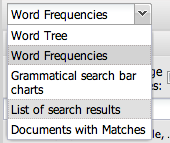
\includegraphics[width=0.2\textwidth]{fig/chris/03.png}
\end{center}
\caption{ The view-switcher drop-down menu.\label{fig:chris03}}
\end{figure}


When a user opens up WordSeer for the first time, instead of  showing a blank screen a requiring the user to think up a query, the tool  provides summary statistics immediately, as shown in Figure \ref{fig:intro01} on a collection of \emph{New York Times} editorials.  Figure \ref{fig:intro02} breaks this down into its core components. This is a single \emph{view} with a \emph{Word Tree} visualization of the most frequent content word in the \emph{slice} consisting of ``the entire collection''. 

\begin{figure}[ht!]
\begin{center}
%
        \subfigure[The initial view for Case Study 1. \label{fig:intro01}]{%
	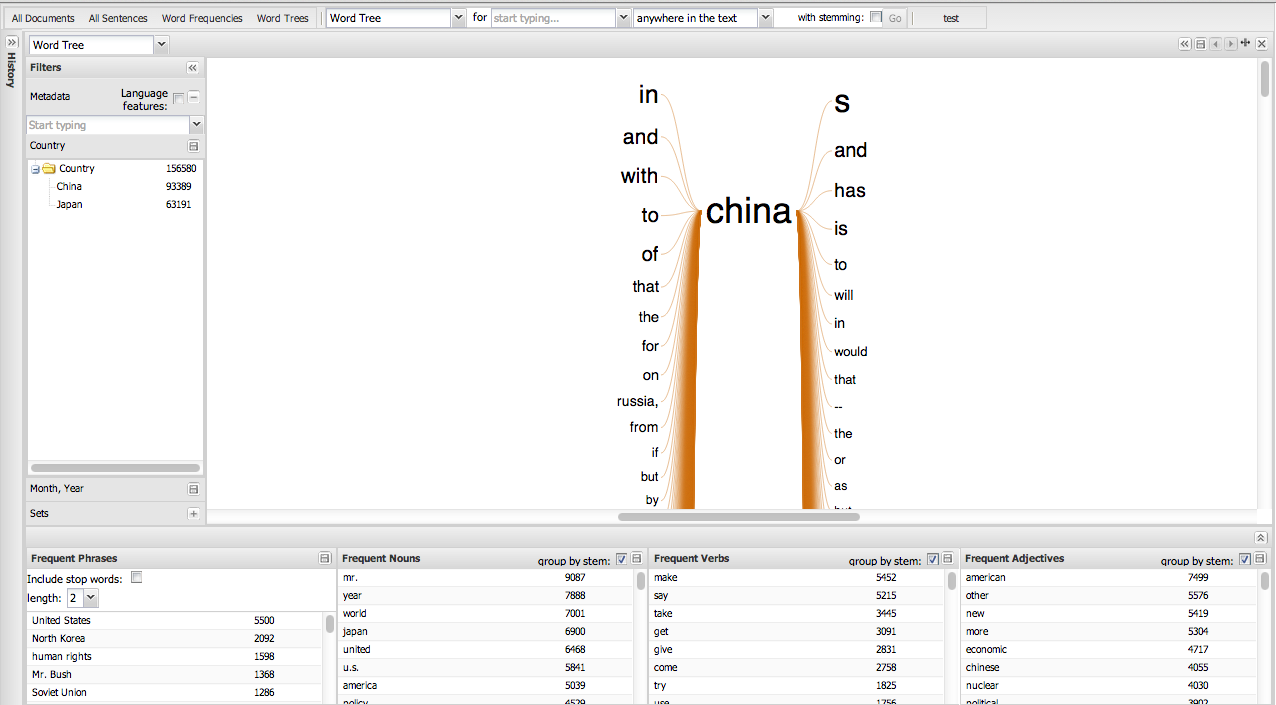
\includegraphics[width=0.5\textwidth]{fig/intro/01.png}
        }%
        \\
        \subfigure[A breakdown of the components of the user interface  \label{fig:intro02}]{%
	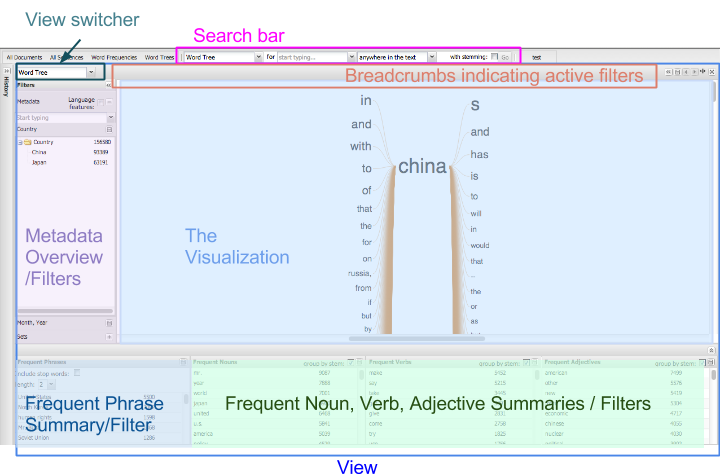
\includegraphics[width=0.5\textwidth]{fig/intro/02.png}
        }%
%
    \end{center}
    \caption{%
       Views in WordSeer.
     }%
\end{figure}

Word Trees \cite{wattenberg_word_2008} are interactive visualizations that allow a user to explore the contexts in which a word is used. They group together common left- and right-contexts into a tree that gets finer and finer as the context get longer, terminating in individual sentences.  Because when the interface is first opened, no query has yet been specified, the Word Tree view centers on the most frequent content word in the collection (content words exclude very common (stop) words, such as ``the'', ``a'', ``and'', etc.). In this case, that word is``China'' (see first case study below).  Other visualizations are also available, including a tabular list of sentences along with their metadata, a heatmap showing the location of query terms within each document, and bar charts and other statistics about the distribution of the metadata and the query terms, as described below.

\subsection{Slices}

The easiest way to make slices in WordSeer is by intersecting \emph{searches} and \emph{filters}.  A search restricts the collection to just the sentences matching the query, and a filter restricts it to just sentences matching a particular metadata value. 

Case study 1 (see below) illustrates the importance of allowing users to compose their own slices. The study was conducted by  C.F.,  a scholar studying US-China relations through a collection of 5,715  \emph{New York Times} editorials about China and Japan from 1980 to 2012. 

One of his first goals was to get a sense of the different ways China was discussed in the `80s, `90s and `00s. To do this, he assembled three slices, one for each decade, by starting with a \emph{search} for ``China'' (Figure \ref{fig:intro03})  and then filtering the `Year' category to range over each ten-year period (Figure \ref{fig:intro04a}).  WordSeer does not require metadata to be numerical ranges, it can also work with categorical values. If he had wanted to, C.F. could have filtered these results to just editorials whose main topic tag was China or Japan, using the controls shown in Figure \ref{fig:intro04b}. 
\begin{figure}[ht!]
\begin{center}
	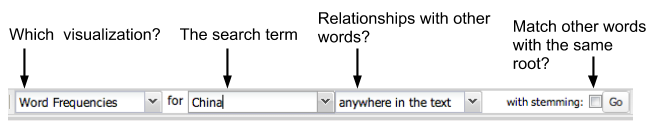
\includegraphics[width=0.5\textwidth]{fig/intro/03b.png}
\end{center}
    \caption{%
        Searching for sentences matching ``China''.\label{fig:intro03}
     }%
\end{figure}

\begin{figure}[ht!]
\begin{center}
%
        \subfigure[C.F. used the date-range overview to select the slice ``all sentences from the 1990's matching \emph{China}'']{%
            \label{fig:intro04a}
	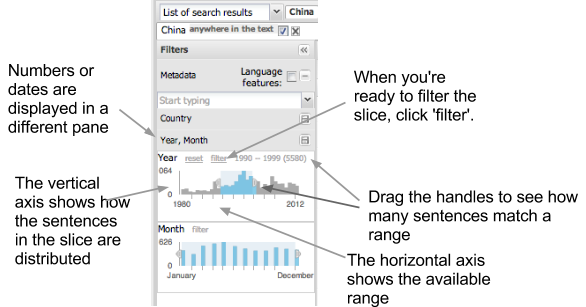
\includegraphics[width=0.5\textwidth]{fig/intro/04b.png}
        }%
        \\
         \subfigure[Clicking on a value will filter the slice to match. For example, clicking on `China' would create the slice  ``all sentences containing \emph{China} from editorials about China''.]{%
            \label{fig:intro04b}
	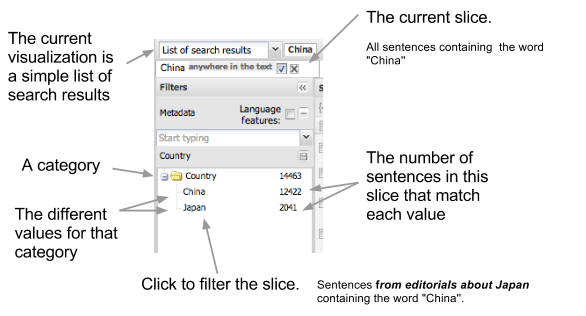
\includegraphics[width=0.5\textwidth]{fig/intro/04a.png}
        }%
%
    \end{center}
    \caption{%
     Both types of overviews double as filters \label{fig:intro04}.
     }%
\end{figure}

WordSeer's overviews showed clear differences between the decades. In particular, the increasing  frequencies of growth-related verbs contributed to a sense of China's rise, as shown by the frequencies per decade below:
\begin{itemize}
\item ``grow, growing'':  294, 232, 421
\item ``rise, rising'': 101, 134, 249
\item ``develop, developing'': 274, 404, 476
\end{itemize}

\subsection{Associated Slices}

 In the database, each sentence is indexed according to the following linguistic phenomena:
\begin{itemize}
  \item Each word in the sentence, and its part of speech (noun, verb, adjective, etc.),
  \item Each consecutive two-, three-, and four-word sequence in the sentence,
  \item Each grammatical relationship in the sentence. 
  \end{itemize}  
 By traversing these indexes, we can compute the associations for a slice. From a slice, we can query for all the words, phrases, or grammatical relations in the sentences in that slice, and from there, to all the other sentences that contain each particular item.  

 Grammatical relationships are identified using the Stanford dependency parser\cite{klein_accurate_2003} which extracts many kinds of relationships; some of the more easily understood ones include \emph{noun compound}, where two nouns come together to signify a new concept, \emph{adjective modifier} where an adjective describes another word, and \emph{direct subject} in which a word is the agent of a verb. 

Each view automatically presents the most common nouns, verbs, adjectives, and phrases (Figure \ref{fig:intro06}),  along with their counts (providing a query preview \cite{donn_query_1996} in a panel at the bottom.    
\begin{figure}[ht!]
\begin{center}
	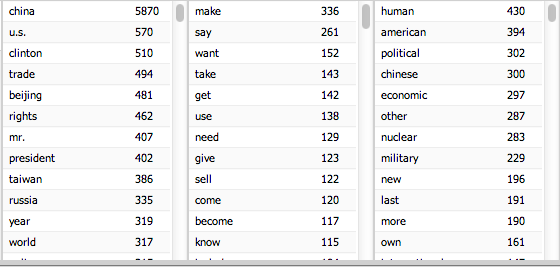
\includegraphics[width=0.5\textwidth]{fig/intro/06.png}
\end{center}
    \caption{%
       The most frequent phrases, nouns, verbs, and adjectives in the \emph{New York Times} editorials for Case Study 1.  \label{fig:intro06}
     }%
\end{figure}

Individual words are jumping-off points. They can be acted upon wherever they appear via the Word Menu (Figure \ref{fig:chris01}) which enables  \emph{lateral movement}.  Any time a user sees a word, they can follow up on it by examining the grammatical relations in which it occurs, seeing related words,  and creating visualizations of the slice of sentences that contains the word, as well as the slices containing various relationships to other words.

\begin{figure}[h!]
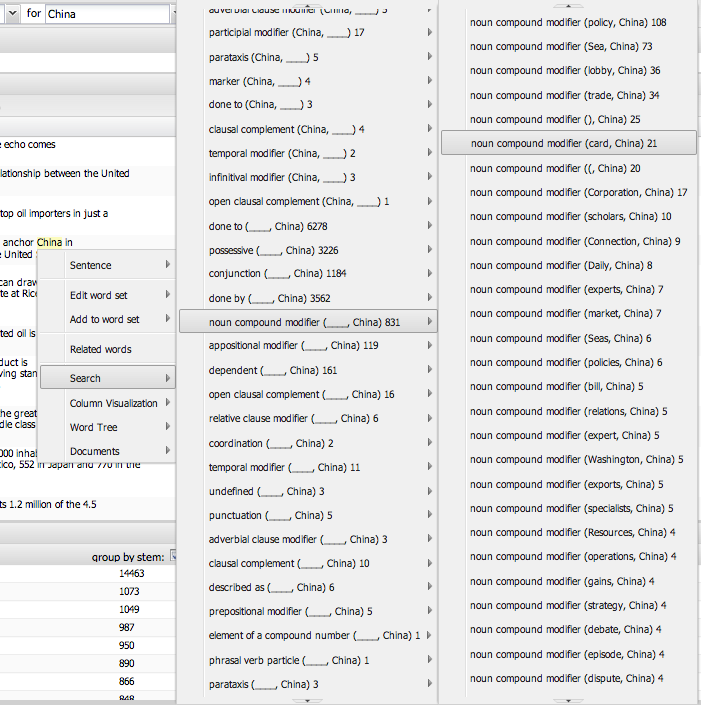
\includegraphics[width=0.5\textwidth]{fig/chris/01.png}
\caption{The word menu for `China'.   After selecting \emph{China > Search > noun compound modifier}, the noun-compound relationship ``China card'' stood out to C.F. \label{fig:chris01}}
\end{figure}


\begin{figure}[ht!]
\begin{center}
	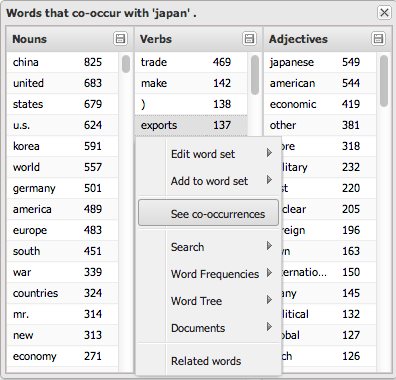
\includegraphics[width=0.3\textwidth]{fig/intro/09.png}
\end{center}
    \caption{%
 		The words that co-occur most frequently with `Japan'. Clicking on any of these words opens up a Word Menu, this time with the option to see the sentences containing the co-occurrence.
	\label{fig:intro09}}%
\end{figure}

The related words option in the Word Menu shows the nouns, verbs, and adjectives that co-occur most frequently with the clicked-on word. For example, if we click on `Japan' and open up the related words (Figure \ref{fig:intro09}) the pop-up shows the words that co-occur most frequently with `Japan' in this collection. Each of these related words can be clicked in turn, opening up a new Word Menu. These menus have the additional option to `See co-occurences', as shown in the new Word Menu for `exports'.  Selecting that option opens up a new view showing just those sentences in which the two words appear together  (in this case, `Japan' and `exports').  

The word menu reduces friction in both discovery and search. It only takes one menu click to discover that `exports' occurs frequently with `Japan', and only one more to see all the sentences in which `Japan' and `exports' are mentioned together.  


\subsection{Custom Slices with Sets}

Searches and filters are useful, but cannot always express  specific analysis goals. WordSeer therefore allows users to construct custom slices through Word-, Sentence-, and Document Sets. These custom slices behave like any other slices, which means that they can be summarized in views,  analyzed, filtered and searched. But they are more powerful that other slices because they also behave like metadata, transforming them into \emph{categorical filters}.

Word Sets are well-illustrated by an example from Case Study 1.  One concept of interest in this study was ``growth''. The scholar wished to confirm his intuitions about China's rise by checking whether  growth-related words became more frequent over time in editorials about China. First, he created a new Word Set and typed in some growth-related words ``growing, develop, developing, grow, rise, rising" (Figure \ref{fig:intro10a-word-sets}). The result was a Word Set representing a new slice of sentences, those containing at least one of those words. 

\begin{figure}[ht!]
\begin{center}
%
        \subfigure[Creating a ``growth'' word set with 6 words in it. \label{fig:intro10a-word-sets}]{%
	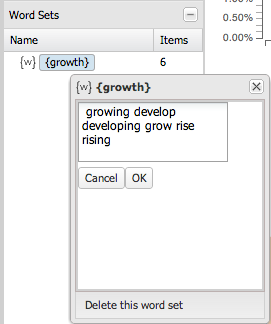
\includegraphics[width=0.2\textwidth]{fig/intro/10a-word-sets.png}
        }%
        \\
        \subfigure[The set now appears in the drop-down menu in the search box. \label{fig:intro10b-word-sets}]{%
	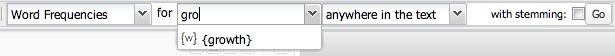
\includegraphics[width=0.5\textwidth]{fig/intro/10b-word-sets.png}
        }%
         \\
        \subfigure[The set also appears in the word menu  \label{fig:intro10c-word-sets}]{%
	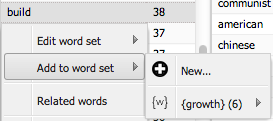
\includegraphics[width=0.2\textwidth]{fig/intro/10c-word-sets.png}
        }%
        \quad
        \subfigure[ The set also appears in the metadata overview   \label{fig:intro10d-word-sets}]{%
	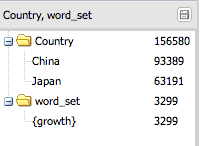
\includegraphics[width=0.2\textwidth]{fig/intro/10d-word-sets.png}
        }%
%
    \end{center}
    \caption{%
       Word Sets in WordSeer. \label{fig:intro10-word-sets}
     }%
\end{figure}
After the Word Set is created, the entire user interface responds to its presence. The search box now shows a drop-down option for the set  (Figure \ref{fig:intro10b-word-sets}).  The Word Menu shows the option to add a new words (Figure \ref{fig:intro10c-word-sets}) and the metadata overviews (Figure \ref{fig:intro10d-word-sets}), previously restricted to pre-defined categories,  now show this new ``category'', and allows C.F. to filter based on it.   

\begin{figure}[ht!]
\begin{center}
	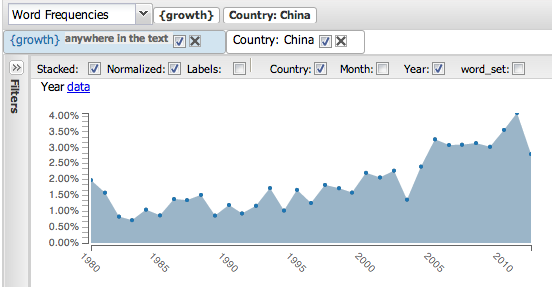
\includegraphics[width=0.5\textwidth]{fig/chris/04a.png}
\end{center}
    \caption{%
	The \code{\{growth\}} Word Set used as a Word Frequencies query.\label{fig:chris04a}
     }%
\end{figure}

To verify that China was indeed described as rising, C.F. selected the  \code{\{growth\}} Word Set as his search query, and opened a Word Frequencies view with the  \code{ country = China} filter. The resulting visualization is Figure \ref{fig:chris04a}, which shows almost a doubling of the frequency of these words in editorials about China over the 30-year period from 1980 to 2012. Satisfied that WordSeer was capable of reproducing this widely accepted fact, he was able to move on to deeper questions.

For sentences and documents, the idea is the same.  Users can hand-pick collections of sentences from the reading view, and from search results view, or collections of documents from the document search results view.  Once created, all these sets can be overviewed and analyzed like any other slice, and additionally used as filters.

This section has introduced the core text sliding features of WordSeer.  The next two sections illustrate them in more depth and show how they were used in two real-world case studies to find information of value to scholar users.

\section{Case Study: U.S. Perceptions of\\China Japan}

As mentioned above, C.F. is a literary scholar at [university's] English department. His work on American literature's reactions to China's rise draws upon a set of historical observations about the ``rise of China'' that are broadly accepted by historians and cultural historians. Literary scholars typically allow their claims to rest on observations made by field experts like historians and sociologists, or on their own inductive reasoning, but C.F. wanted to verify some of those observations by gathering as much empirical evidence for them as possible. 
 
Using the Lexis/Nexis database, C.F. collected \emph{New York Times} editorials from 1980 to 2012, limiting his collection to editorials tagged with subjects ``China" or ``Japan." This left a set of 5,715 editorials, which we imported to WordSeer. Each editorial was associated with three pieces of metadata: year, month, and country (either China or Japan).

After a few weeks of face-to-face meetings, C.F. gradually became comfortable using WordSeer on his own.  He used WordSeer to find evidence for discussion of the rise of China as described above, and for three other hypotheses, two of which are described below.

\subsection{1980's: China Insignificant Except for Cold War Strategy}
While comparing the most frequent adjectives for the three decades, C.F noticed a drop-off in cold war words. ``Soviet''  went from  a count of 1029 in the 1980's to only 80 in the 2000's, and ``communist'' went from 284 to 112.   To investigate the drop-off in more detail, he used the the Word Menu to quickly open up word frequency plots for these two words over time, and filtered them to just the editorials about China.  Figure \ref{fig:chris04b} shows a plot of these words together:

\begin{figure}[h!]
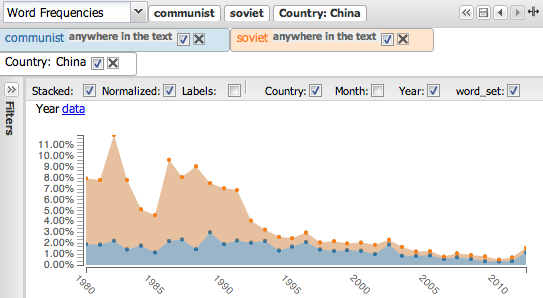
\includegraphics[width=0.5\textwidth]{fig/chris/04b.png}
\caption{The frequencies of `communist' (blue) and `soviet' (orange) in editorials about China over time. \label{fig:chris04b}}.
\end{figure}

Plotting the terms together (Figure \ref{fig:chris04b}) added depth to his initial calculations.  The plot shows the dominance, and equally dramatic drop-off, in cold war mentions over this time period. In the early 1980's, almost 11\% -- more than 1 in 10 sentences in those editorials -- mentions one of these the cold war terms. By the 1990's, however, this association is down to a trickle. 

An exploration of the ``grammatical neighborhood'' around `China'  helped C.F. find yet more evidence for this idea. This time, it was through a distinctive rhetorical device. As Figure \ref{fig:chris01} shows, clicking on the word ``China'' opens up a menu with search options. These options act as quick previews of different grammatically-related slices: they show the frequencies with which ``China'' occurs in different grammatical constructions with different words.  For C.F., the noun compound relationship yielded a surprise. He noticed an odd construction, ``China card,'' which appeared 21 times.

He immediately explored this this distinctive usage by selecting List of Search Results options for that relationship.  This opened up the list of sentences in which the noun compound ``China card'' occurred.  When C.F. read the sentences, an interpretation suggested itself:
\begin{quote}
[Reading] the sentence search results reveals that phrase is used to refer to the China's strategic value in Cold War geopolitics. Of the four post-2000 instances, only one uses the phrase to describe a contemporary political situation; the others use it to describe Cold War politics. Reducing the vastness of China to a disposable ``card,'' indicates a degree of U.S. self-confidence, not to mention condescension, that disappears after 1989.
\end{quote}

The Word Frequencies view of the same data allowed him to make that temporal claim. Using the drop-down menu at the top left of the panel (Figure \ref{fig:chris03}) he opened up the word frequencies view alongside his list of search results.  Because the ``year'' metadata was attached to each article, this view displayed a graph of how frequent  sentences containing ``China Card'' were over time (Figure \ref{fig:chris02}). 
\begin{figure}[h!]
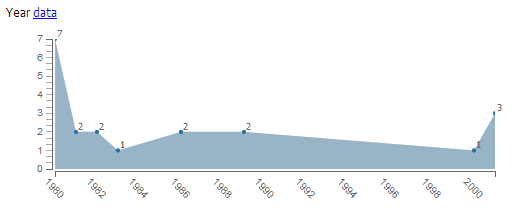
\includegraphics[width=0.5\textwidth]{fig/chris/02.png}
\caption{ The number of sentences matching ``China card'' over time. \label{fig:chris02}}
\end{figure}
The graph shows that ``China card'' the rhetorical figure signifying cold-war strategic value, was used relatively frequently until 1989, but rarely  after that. This supported his claim that, up until the early 90's, China had a Cold-war strategic significance to the U.S. that later dissipated.

\subsection{Mid 1990's onwards: China's ties with the U.S. Strengthen}

A major event in Chinese international relations occurred in 2001, when China joined the World Trade Organization (WTO).  Although attention had been shifting towards China since the 1990's, it is during this period that U.S.-China relations are thought to have become more interdependent, and central to global politics. 

To find evidence for this, C.F.  started with a grammatical structure he thought might make a good proxy for U.S.-China relations: the \emph{conjunction}, which is just an \emph{and} relationship between two words.  He needed a grammatical search because of the possibility of constructions like 
\begin{quote}
``The United States, the world's top energy guzzler, and China, with the world's fastest-growing energy thirst \ldots" (April 2006).
\end{quote}
This fragment places China and the United States in clear conjunction with each other, but an exact-phrase search for \code{`United States and China'} would miss it. 

He created a list of search results view, containing a total of 142 sentences (Figure \ref{fig:chris05}).
\begin{figure}[h!]
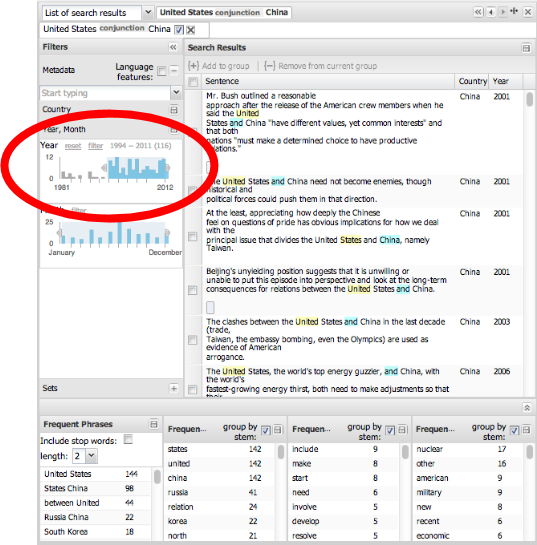
\includegraphics[width=0.5\textwidth]{fig/chris/05-circled.png}
\caption{ A \emph{List of Search Results} view of the \code{conjuction(United States, China)} sentences. \label{fig:chris05}}
\end{figure}
A quick look at the distribution of articles over the Year category (circled in red) confirmed his choice of starting point. These were much more frequent from the mid-nineties onward. In fact, out of the 142 occurrences, 116 (81\%) occurred after 1994.

He began skimming over the results, but soon noticed a problem. While these these sentences did indeed contain many references to U.S.-China relations, they also contained many conjunctions that weren't interesting: purely grammatical ones like ``While maintaining cautious vigilance against rival powers, the United States, Soviet Union, and China separately welcomed this trend.'', and relations involving other parties, like ``In turn, the nuclear five -- the United States, Britain, Russia, France and China -- committed themselves to sign a comprehensive test ban by next year.''

WordSeer's sentence sets are designed to solve this problem. C.F. recognized this, and put them to use. He manually inspected each of the 134 results, and created a sentence set out of the ones that satisfied his criteria: having to do with relations solely between the U.S. and China relations.  He called this set \code{\{US-China relations\}}. Sentences were sometimes ambiguous, but the ease of looking up the sentence within the editorial made it easy to check whether or not it should be included. To quote:
\begin{quote}
[The filtering process] was significantly aided by the ability to click on the sentence and immediately see it located in context within the full editorial.
\end{quote}
He eliminated about half the sentences from consideration, leaving him with a set of  79 sentences. A Word Frequencies view of this smaller slice made the picture much clearer. Of the 79 sentences, the overwhelming majority (86\%) occurred after 1995.

C.F. noticed a subtle point: as he moved from the 1990's to the 2000's, the relationship between the U.S. and China seemed to be increasingly  `central' and `inter-dependent':
\begin{quote}
Phrases and words like the following begin to appear: ``21st century's most important relationship,'' ``co-dependent,'' ``interlocking,'' etc. But I achieved a more precise sense of the themes of \emph{interdependence} and \emph{centrality } more precisely using a Word Set of thematically-related adjectives drawn from the Frequent Adjectives overview.
\end{quote}
C.F. composed a Word Set of words from the overview, consisting of: ``most, central, important, indispensable, dependent, interdependent, dependency, entangled, interlocking, interdependency''.   Figure \ref{fig:chris07} shows the distribution of centrality and interdependence adjectives detected automatically by the tool, intersected with the conjoined U.S.-China relationship sentences curated by C.F. The year-overview for the filtered set immediately shows that it is not until 1995 that the U.S.-China relationship is characterized by these themes.

\begin{figure}[h!]
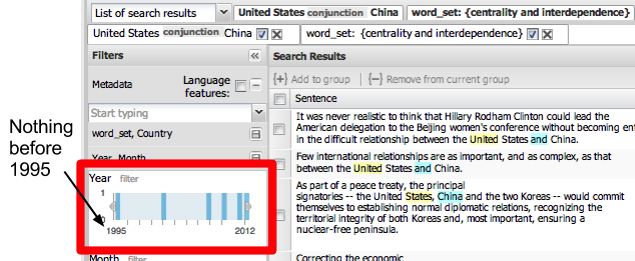
\includegraphics[width=0.5\textwidth]{fig/chris/07.png}
\caption{ The distribution of the \code{\{centrality and interdependence\}} Word Set within the \code{conjunction(United States, China)} slice. There are no occurrences before 1995. \label{fig:chris07}}
\end{figure}


\section{Case Study: Literacy Essays}

\subsection{Introduction}
As a college English Composition instructor,  R.G., at  [university's] school of Education asks students to write often and in a variety of situations. In this project, he examined ways in which WordSeer could assist him in the teaching and learning of writing. He was particularly interested in the literacy autobiography, in which students describe significant experiences they have had with literacy and reflect upon the importance of literacy to their lives.  

R.G. analyzed the content of approximately 140 literacy autobiographies written by students from courses that he has taught over that past two years, each about 1,500 to 2,000 words long. He is familiar with the collection, having previously read and commented on each of the essays.  Table \ref{table:rex-courses} shows the different courses from which literacy autobiographies were analyzed. The courses were at different colleges and taught at different proficiency levels.

Among the questions that guided his inquiry were the following. In this example, we show how the tool helped him get answers:
\begin{enumerate}
\item What can a distant reading of student literacy autobiographies tell him about students that close readings cannot?
\item What patterns exist in student literacy autobiographies at different course levels and institutions?
\end{enumerate}

\begin{table}
\begin{tabular}{lll}
Course& College & Level \\
\hline
Engl 1A (n=29) & [anonymized] & First-year \\
Engl 201AB (n=28) & [anonymized] & Pre-transfer \\
Engl 5 (n=40) & [anonymized] & Transfer level \\
Edu 140 (n=40) & [anonymized] & Upper division \\
\end{tabular}
\caption{The four different courses, each at a different proficiency level, from which literacy autobiographies were analyzed by R.G. \label{table:rex-courses}}
\end{table}


 \subsection{A new take on students' experiences}

R.G. does not usually consider the frequencies of words unless a student repeats one to the point of distraction. However, the WordSeer's very first overview (automatically generated for the whole collection on startup) prompted him to consider the significance of individual words and their repeated use.  As he states:
\begin{quote}
From the moment I opened WordSeer, `distance' immediately provided new insight and areas of exploration as I was intrigued by unexpected high word frequencies.  The most obvious example is the frequent use of the word ``time" which is not only the most frequent noun but also the most frequent word overall.  As opposed to ``literacy'', ``language'', and any noun or verb forms of ``read'' and ``write'', the Word Tree for ``time'' appears before any term is placed in the keyword search.   I found similar surprises in the adjective and verb frequencies, and these surprises would guide my decision-making and analysis.
\end{quote}
Faced with unexpected discoveries in every part of speech, R.G. decided to explore the adjectives. The top three adjectives were not surprising - ``other" (474),``first" (379), and ``new" (384).  However,  ``able'' (314) and ``own'' (282) were words that he did not expect to be used frequently.

R.G. now wanted to understand the unexpectedly high frequencies of ``able'' and ``own''. WordSeer made this exploration easier. Instead of having to open a new window and type new search queries, clicking on the words themselves opened up Word Menus which allowed him to create Word Trees centered on those words.

\begin{figure}[h!]
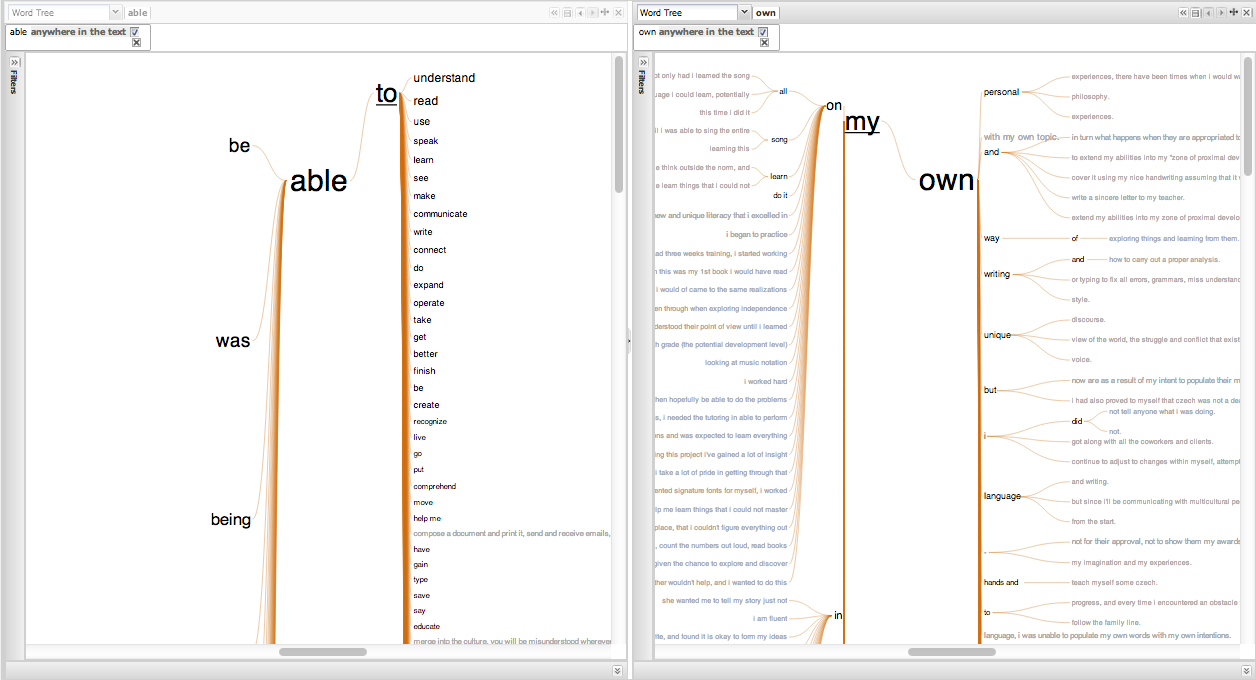
\includegraphics[width=0.5\textwidth]{fig/rex/04.png}
\caption{ Side-by-side Word Trees (with overview panels collapsed) for `able' and `own', created from the Word Menu. \label{fig:rex04}}
\end{figure}

The Word Tree for ``able" (Figure \ref{fig:rex04} left) revealed that the most common use of the adjective able was: \code{[form of the verb `to be'] + able + to [action verb]}. To get a sense of how common this usage was overall, R.G. hovered over each branch (which displayed the number of sentences under that branch), and adding up the numbers for branches matching ``to be''. He found that the overwhelming majority, 280 out of 314 occurrences, fell into this pattern, with the most common ``abilities'' being literacy-related: read, understand, communicate, learn, speak, etc. For  ``own'' (Figure \ref{fig:rex04} right), the most common construction was: \code{[preposition] + my + own}, with around a third: 100 out of 291 occurrences.  He also used the Word Tree to zoom in and read the individual sentences.

As a result, R.G. came away with a new insight about his students:
\begin{quote}
Student writers articulate their experiences from some first encounter with the unfamiliar, followed by a process of being ``able" to act within that which is becoming less unfamiliar.  Moving into literacy requires these writers to develop their ``own" abilities as necessary to survive and prosper in that context.
\end{quote} 

\subsection{Writing proficiency across courses}
The different courses R.G. taught were taken by students with differing amounts of college education. He was especially interested in differences in sentence construction, hypothesizing that more proficient students would use advanced structures more frequently. To initiate the analyses, he performed word searches on terms such as ``though", ``while", ``although", and ``however", which indicate a complex structure called a ``concessive''. He was expecting concessives to be increasingly frequent as student experience increased from English 1A, to English 201, to English 5, to Ed140.

To follow up R.G. created a Word Frequencies visualization of this terms. This visualization shows how often terms occur across different metadata categories (and can show the counts stacked or grouped, normalized or raw). R.G. added all the concessive terms to the same view, which created a comparative visualization (Figure \ref{fig:rex05}).
\begin{figure}[h!]
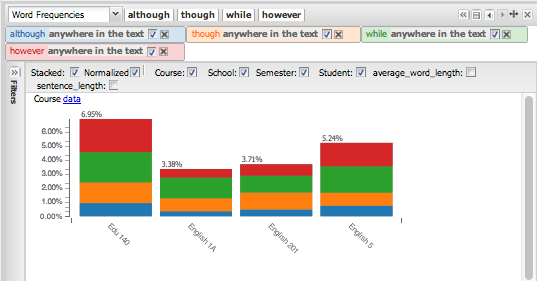
\includegraphics[width=0.5\textwidth]{fig/rex/05.png}
\caption{The frequencies of different "concessive" words across the Course category: `although' (blue), `though' (orange) `while' (green) and `however' (red). \label{fig:rex05}}
\end{figure}
The increasing frequencies across the course levels confirmed his hunch that as students become more experienced and comfortable with the written word, they used more complex sentence structures more frequently. 

\section{Discussion}
The case studies show how WordSeer's text manipulation and visualization features helped scholars make new discoveries about the world and create new understanding from text collections; these are discoveries that most likely would not have been able to make with any other existing tool.

Prior to using WordSeer, C.F. had general ideas about the points he wanted to make based on years of reading, but had no way to quantify or codify those ideas based on data.  In just a few weeks, WordSeer allowed him to find changes in use in language that reflected historians' understanding of the rise of China (its transformation from a `card' played by American diplomats during the cold war,  to its present-day status as a `central' and `entangled' partner of the United States), but with more precision (the steady increase in growth-related verbs over the last 30 years, the sudden jump in  phrases like ``US and China'' after 1994) and with more nuance (the emergence of words relating to the `centrality' and `interdependence'  of their relationship in the 2000s).

Prior to using WordSeer, R.G. had spent hours reading and thinking about the literacy essays, but had not looked at them in terms of word frequency or syntactic structure.  Using WordSeer, he was able to see the documents in a new light and form new  understanding of the general trends in his students' process of learning to write.   He was also able to formulate and find evidence for a hypothesis about an increase in proficiency with advanced writing structures as they moved to successively advanced educational levels.   He used a complex combination of searching for grammatical structures, side-by-side comparisons of sets of sentences according to adjectives and their use in context, selecting a subset of words and comparing their frequency across a metadata classification.  

A key component of the use of the tool in these examples is the freedom it affords the user to pivot on words, on words' relations to other words, to create groups of words and cross them with arbitrary metadata categories, and to be able to immediately view  the context of their original sentences and documents, thus allowing ``close reading" as part of the text analysis process.

\section{Future Work}
As an exploratory data analysis (EDA) system, WordSeer aids in the formulation of hypotheses, and the accumulation of evidence in favor or in refutation of hypothesis. A significant improvement to the tool would be a way to help users try to disprove any hypothesis that they think the tool has helped them to find. For example, assessments of literacy essays could be compared to learning outcomes and grades.

There are several improvements that need to be made to the user interface. The most pressing problem is the rigid left-to-right arrangement of panels, which makes having more than two or three simultaneous views impractical on most displays. A more adaptive, customizable layout would make managing and navigating between views more frictionless. Next, the user's history of actions should be made more accessible. At present history is presented as a linear sequence of actions. The system should instead give the user a sense of the different sensemaking paths they have taken, and allow them to replay their history, and branch off from it.

The third problem is that users cannot customize their views according to their needs. The same three overviews are always present: the metadata on the left, and the most frequent phrases, nouns, verbs, and adjectives on the bottom. The user should be able to choose to expand or collapse these by default, as well to choose different overviews: perhaps the most most distinctive words in the slice, instead of the most frequent. The overviews also need to make it clear that the the counts they show are the number of matching \emph{sentences}, and not the number of matching \emph{documents}, and to give users a way of switching between the two.

Finally, although the tool provides results in under a second in some cases, in other cases the wait is longer, depending on the size of the collection and the operation requested.  A next step will be optimizing of the tool's performance to further encourage exploration. 
 
 \subsection{Requested Features}
 Both scholars wanted to search for sentence structures beyond word-to-word relationships. C.F. was interested in sentences with a comparative structure, specifically comparisons between  Chinese and Japanese things. As a composition instructor, R.G. was interested in applications of a ``sentences structure search'' to teaching.  If there was a way to summarize students' most frequent sentence-structure mistakes, or to find overall commonalities in the ways students structured their sentences, instructors could focus on helping the students improve in those areas.
 
Both scholars also wanted to automatically create groups based on a set of examples, and to fine-tune the results by giving feedback. For example, C.F. could have used it to identify sentences describing the complexities of the US-China relationship, and R.G. could have used it to automatically catalog the different senses of the word ``get'':  becoming (`I got ready to \ldots'), and acquisition (`I got a lot of practice \ldots'). Instead of having to manually construct them by reading.
 
The system should also incorporate standard text analysis tools such as text classification and sentiment analysis, and should allow users to make organize words according to pre-defined word dictionaries.

\bibliographystyle{abbrv}
\bibliography{old_cikm} 
  
\end{document}


